%!TEX TS-program = xelatex
\documentclass{EdipyLabs} % Custom class provided for EDIPY labs, by Christos Dalamagkas (cdalamagkas@gmail.com)
\SetLabNumber{1β}
\SetLabTitle{Εισαγωγή στο RouterOS}
\SetAuthor{Χρήστος Δαλαμάγκας}
\SetLabDescription{MikroTik, RouterOS, CLI, υποκατάλογοι, σύνδεση στο τερματικό, βασικές εντολές.}
\SetLabPrerequisites{Βασική ορολογία δικτύων υπολογιστών, στοιχειώδης εξοικείωση με λειτουργικά συστήματα Unix.}

\begin{document}

\Initialize

\section{RouterOS}
To \textbf{RouterOS} είναι το λειτουργικό σύστημα της εταιρείας MikroTik, βασισμένο σε πυρήνα Linux, το οποίο χρησιμοποιείται για τη λειτουργία των δρομολογητών και μεταγωγέων της εταιρείας. Σε αντίθεση με λειτουργικά συστήματα άλλων εταιριών, όπως το Cisco IOS και το AlliedWare OS, το RouterOS διατίθεται δωρεάν προς λήψη και έχει τη δυνατότητα να εγκατασταθεί σε οποιονδήποτε υπολογιστή ή εικονικό μηχάνημα ως αυτόνομο λειτουργικό σύστημα. Ουσιαστικά, το RouterOS μπορεί να μετατρέψει οποιονδήποτε υπολογιστή με δυο ή περισσότερες NIC σε ισχυρό δρομολογητή με υποστήριξη δυναμικής δρομολόγησης, τείχους προστασίας, κλπ. 

\subsection{Διεπαφή Χρήστη}
Η διεπαφή γραμμής εντολών (Command Line Interface - CLI), αποκαλούμενη ως «κονσόλα» από την MikroTik, είναι το βασικό περιβάλλον χειρισμού του RouterOS. To CLI του λειτουργικού συστήματος προσφέρει εκατοντάδες εντολές, οι οποίες ακολουθούν ένα ιεραρχικό μοντέλο με κατάλογους και υποκατάλογους. H γενική μορφή μιας εντολής στο CLI του RouterOS απεικονίζεται στο σχήμα \ref{fig:command-structure}.

\begin{figure}[H]
	\centering
	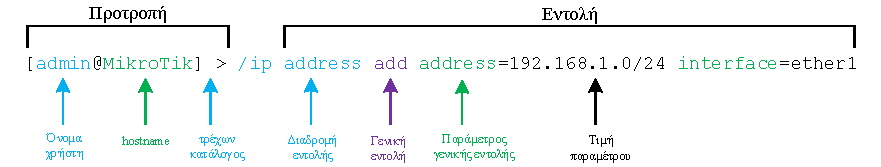
\includegraphics[width=\textwidth]{command-structure}
	\caption{Η μορφή μιας εντολής στο CLI του RouterOS}\label{fig:command-structure}
\end{figure}

Η προτροπή του CLI αποτελείται από το όνομα του χρήστη που έχει κάνει login, το όνομα της συσκευής (hostname) και τον τρέχοντα κατάλογο στον οποίο βρίσκεται η συνεδρία. Αρχικός κατάλογος στην εκκίνηση μιας συνεδρίας είναι η ρίζα ( \texttt{/} ), η οποία δεν εμφανίζεται στην προτροπή όταν ο χρήστης βρίσκεται εκεί. 

Μια τυπική εντολή στο CLI αποτελείται από τον προσδιορισμό της διαδρομής από τον τρέχοντα κατάλογο (path), τη γενική εντολή (general command), καθώς και ορισμό παραμέτρων που δέχεται η γενική εντολή. Η εντολή του παραδείγματος αναθέτει διεύθυνση IP σε μια διεπαφή.

Το CLI χρησιμοποιεί χρωματικούς κώδικες ώστε να διακρίνονται οι διαδρομές των υποκαταλόγων από τις γενικές εντολές. Συγκεκριμένα, οι κατάλογοι και υποκατάλογοι χρωματίζονται με γαλάζιο χρώμα και οι γενικές εντολές με μοβ.

Οι βασικότεροι κατάλογοι του RouterOS που βρίσκονται στη ρίζα συνοψίζονται στους εξής:
\begin{itemize}
	\item \ip{/interface}: Προβολή και παραμετροποίηση των διεπαφών της συσκευής. Οι εμπεριεχόμενοι υποκατάλογοι και εντολές εστιάζουν σε λειτουργίες επιπέδου 2 του OSI (ζεύξης δεδομένων).
	\item \ip{/ip}: Περιέχει υποκαταλόγους και εντολές που σχετίζονται με το IPv4 και περιλαμβάνουν από το επίπεδο 3 (δικτύου) μέχρι και το επίπεδο εφαρμογών του OSI. 
	\item \ip{/ipv6}: Αντίστοιχοι υποκατάλογοι και εντολές με τον κατάλογο ip, αλλά για το ipv6. 
	\item \ip{/routing}: Εντολές και υποκατάλογοι σχετικά με πρωτόκολλα δυναμικής δρομολόγησης.
	\item \ip{/system}: Εντολές και υποκατάλογοι σχετικά με παραμετροποίηση του συστήματος RouterOS.
	\item \ip{/tool}: Χρήσιμα δικτυακά εργαλεία για έλεγχο του συστήματος και του περιβάλλοντός του.
\end{itemize}

Περισσότερες λεπτομέρειες για τους παραπάνω κατάλογους μπορείτε να βρείτε και στο wiki της MikroTik: \url{https://wiki.mikrotik.com/wiki/Manual:TOC}.

\subsection{Μέθοδοι πρόσβασης στο CLI}
H πρόσβαση στο CLI μπορεί να γίνει με τις εξής μεθόδους:
\begin{itemize} 
	\item [\textbf{Console}:] Η κονσόλα αποτελεί τη φυσική θύρα διαχείρισης, συνήθως υπό μορφή σειριακής θύρας, η οποία παρέχει πρόσβαση \textit{out-of-band} σε μια συσκευή. Ο όρος out-of-band αναφέρεται στη χρήση ενός αποκλειστικού καναλιού που προορίζεται για τη διαχείριση της συσκευής.
	\item [\textbf{SSH}:] Αν δεν υπάρχει φυσική πρόσβαση στο μηχάνημα, είναι δυνατή η απομακρυσμένη σύνδεση σε αυτό μέσω του πρωτοκόλλου SSH, το οποίο παρέχει ασφαλή σύνδεση στο κέλυφος βασιζόμενο στη μέθοδο κρυπτογράφησης δημόσιου κλειδιού. Προϋπόθεση για τον συγκεκριμένο τύπο σύνδεσης είναι η ενεργοποίηση των απαραίτητων υπηρεσιών δικτύωσης, συμπεριλαμβανομένης μιας ενεργής διεπαφής με διεύθυνση IP. Η μέθοδος αυτή, όπως και η Telnet, αποκαλούνται \textit{in-band}, διότι χρησιμοποιούν ήδη υπάρχοντα κανάλια επικοινωνίας.
	\item [Telnet:] To πρωτόκολλο telnet επιτρέπει και αυτό απομακρυσμένη διαχείριση, όπως το SSH, με τη διαφορά ότι δεν υποστηρίζει κρυπτογράφηση, με αποτέλεσμα ευαίσθητες πληροφορίες όπως κωδικοί πρόσβασης να μεταδίδονται ως καθαρό κείμενο. Η χρήση του δεν συνίσταται.
\end{itemize}

Η σύνδεση με το CLI μπορεί να εγκαθιδρυθεί είτε με κάποιο κλασικό πρόγραμμα εξομοίωσης τερματικού, όπως το PuTTY, ή με την εφαρμογή Winbox που διατίθεται δωρεάν από την MikroTik αποκλειστικά για τη σύνδεση και τον χειρισμό μηχανημάτων (εικονικών ή φυσικών) που εκτελούν RouterOS. Περισσότερα για το Winbox μπορείτε να βρείτε στο Wiki της Mikrotik: \url{https://wiki.mikrotik.com/wiki/Manual:Winbox}. H εφαρμογή είναι διαθέσιμη για λήψη στη διεύθυνση: \url{https://mikrotik.com/download}.

Για να συνδεθείτε μέσω PuTTY, συνδέστε το σειριακό καλώδιο Female/Female στη θύρα κονσόλας και το άλλο άκρο του σειριακού καλωδίου με τον μετατροπέα Serial-to-USB. Αφού βρείτε τη θύρα COM που αντιστοιχεί ο μετατροπέας Serial-to-USB παραμετροποιήστε το PuTTY όπως φαίνεται στην εικόνα \ref{fig:putty}. Το προεπιλεγμένο όνομα χρήστη είναι \textbf{admin}, χωρίς κωδικό πρόσβασης.

\begin{figure}[H]
	\centering
	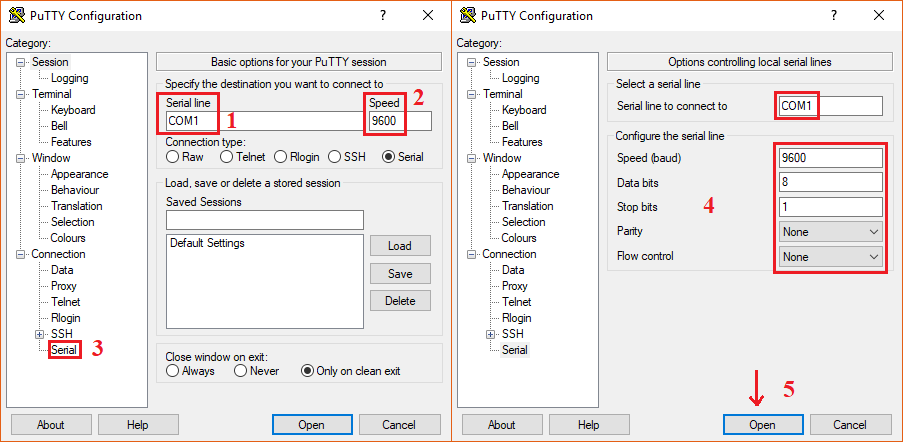
\includegraphics[width=0.8\textwidth]{putty}
	\caption{Η παραμετροποίηση του PuΤΤΥ για σύνδεση σε συσκευή MikroTik.}\label{fig:putty}
\end{figure}

\subsection{Αποθήκευση, ανάκτηση και επαναφορά ρυθμίσεων}
Σε αντίθεση με το Cisco IOS, οι αλλαγές ρυθμίσεων που γίνονται στο RouterOS παραμένουν σε περίπτωση που επανεκκινηθεί η συσκευή. Ωστόσο, αποτελεί σημαντική υπόθεση η διαδικασία αποθήκευσης και ανάκτησης των ρυθμίσεων σε περιπτώσεις πειραματισμών που μπορεί να οδηγήσουν σε ανεπιθύμητα αποτελέσματα. Ο κατάλογος στον οποίον γίνεται ο χειρισμός των backup είναι ο \texttt{/system backup}.

Η αποθήκευση των τρεχουσών ρυθμίσεων σε αρχείο με το όνομα \texttt{test} γίνεται με την εντολή:

\begin{CommandBox}
[admin@MikroTik] > `\textbf{/system backup save name=test}`
\end{CommandBox}

Από προεπιλογή, τα αρχεία ρυθμίσεων αποθηκεύονται στον κατάλογο \texttt{/file} με την κατάληξη .backup. Μπορείτε να προβάλλετε τα περιεχόμενα του καταλόγου με την εντολή \texttt{/file print}

\begin{CommandBox}
[admin@MikroTik] > `\textbf{file print}`
\end{CommandBox}

Η ανάκτηση των ρυθμίσεων από το αρχείο test μπορεί να γίνει με την εντολή \texttt{/system backup load} προσδιορίζοντας στην παράμετρο \texttt{name} το όνομα του αρχείου.

\begin{CommandBox}
[admin@MikroTik] > `\textbf{system backup load name=test}`
Restore and reboot? [y/N]:
`\textbf{y}`
Restoring system configuration
System configuration restored, rebooting now
\end{CommandBox}

H επαναφορά στις εργοστασιακές ρυθμίσεις γίνεται με την εντολή \texttt{/system reset-configuration}:

\begin{CommandBox}
[admin@MikroTik] > `\textbf{system reset-configuration}`
\end{CommandBox}

\subsection{Απαρίθμηση διεπαφών}

Οι διεπαφές ethernet της συσκευής MikroTik απαριθμούνται από το 1 μέχρι το 8 με την ονομασία \texttt{etherX}, δηλαδή \texttt{ether1}, \texttt{ether2}, ..., \texttt{ether8}, με την αρίθμηση να ξεκίνα από τα αριστερά προς τα δεξιά.

\subsection{Περιήγηση στο CLI του RouterOS}

Πληκτρολογώντας μόνο τη διαδρομή, χωρίς κάποια γενική εντολή, μπορείτε να μεταφερθείτε στον επιθυμητό κατάλογο και από εκεί να πληκτρολογείτε εντολές του συγκεκριμένου υποκατάλογου χωρίς να προσδιορίζετε την πλήρη διαδρομή. Για παράδειγμα, η εκτύπωση του πίνακα δρομολόγησης μπορεί να γίνει και ως εξής:

\begin{CommandBox}
[admin@MikroTik] > `\textbf{ip route}
[admin@MikroTik] /ip route> `\textbf{print}
...
\end{CommandBox}

Με τις διπλές τελείες (..) μπορείτε να επιστρέψετε στον αμέσως προηγούμενο κατάλογο:

\begin{CommandBox}
[admin@MikroTik] /ip route> `\textbf{..}`
[admin@MikroTik] /ip>
\end{CommandBox}

Για να επιστρέψετε στη ρίζα μπορείτε να δώσετε την εντολή \texttt{/}:

\begin{CommandBox}
[admin@MikroTik] /ip route> `\textbf{/}`
[admin@MikroTik] >
\end{CommandBox}

\subsection{Λειτουργίες βοήθειας του RouterOS και διευκόλυνση πρόσβασης}
Η υπηρεσία βοήθειας του RouterOS για έναν υποκατάλογο ή εντολή παρέχεται με τον χαρακτήρα \texttt{?}. Το κείμενο βοήθειας μπορεί να εμφανιστεί πληκτρολογώντας την εντολή για την οποία ο χρήστης ζητά πληροφορίες και μετά το ερωτηματικό. Οι πληροφορίες που εμφανίζονται αφορούν, καταρχάς, την ίδια εντολή ή υποκατάλογο, καθώς και τους διαθέσιμους υποκατάλογους ή εντολές που είναι διαθέσιμες. 

\begin{CommandBox}
[admin@MikroTik] > `\textbf{ip address ?}`
IP addresses are given to router to access it remotely and to specify it as a gateway for other hosts/routers.

.. -- go up to ip
add -- Create a new item
comment -- Set comment for items
disable -- Disable items
edit -- 
enable -- Enable items
export -- Print or save an export script that can be used to restore conf
find -- Find items by value
get -- Gets value of item's property
print -- Print values of item properties
remove -- Remove item
set -- Change item properties

[admin@MikroTik] >
\end{CommandBox}

Όπως και με το Cisco IOS, το CLI του RouterOS δίνει τη δυνατότητα στον χρήστη να εκτελέσει μια εντολή με χρήση του ελάχιστου πλήθους χαρακτήρων που τη διακρίνουν μοναδικά. Για παράδειγμα, η εντολή \texttt{ip route print} εκτελείται και ως \ip{ip r p}. H σύντμηση μπορεί να εφαρμοστεί σε οποιαδήποτε λέξη αποτελεί την εντολή, αρκεί να μην δημιουργείται ασάφεια, όταν μια σύντμηση ταυτίζεται με περισσότερες επιλογές. Για να προσδιορίσετε τις λέξεις με τις οποίες ταυτίζεται μια σύντμηση, μπορείτε να πληκτρολογήσετε τη σύντμηση πατώντας δυο φορές το πλήκτρο Tab. Για παράδειγμα:

\begin{CommandBox}
[admin@MikroTik] > `\textbf{ip route e} \textit{[Tab][Tab]}`
edit  enable  export
[admin@MikroTik] >
\end{CommandBox}

Τέλος, το RouterOS παρέχει πλήθος συνδυασμών πλήκτρων για τη διευκόλυνση πρόσβασης στο CLI. Ο πλήρης κατάλογος των συνδυασμών είναι διαθέσιμος στο Wiki της MikroTik: \url{https://wiki.mikrotik.com/wiki/Manual:Console}.

\subsection{Ονόματα και αριθμοί αντικειμένων}
Πολλοί υποοκατάλογοι λειτουργούν με λίστα αντικειμένων, τα οποία προβάλλονται σε αριθμημένη τάξη δίνοντας την γενική εντολή \texttt{print}. Κάθε αντικείμενο σε έναν υποκατάλογο εμφανίζεται με τον αριθμό του, ακολουθούμενο από διάφορες ιδιότητες που το χαρακτηρίζουν. Για παράδειγμα, η εντολή \texttt{ip address print} τυπώνει τις διευθύνσεις που έχουν ανατεθεί στις διεπαφές του δρομολογητή:

\begin{CommandBox}
[admin@MikroTik] > `\textbf{ip address print}`
Flags: X - disabled, I - invalid, D - dynamic
#   ADDRESS            NETWORK         BROADCAST       INTERFACE
0   2.2.2.1/24         2.2.2.0         2.2.2.255       ether2
1   10.5.7.244/24      10.5.7.0        10.5.7.255      ether1
2   10.10.10.1/24      10.10.10.0      10.10.10.255    ether2
[admin@MikroTik] > 
\end{CommandBox}

Όπως φαίνεται στο αποτέλεσμα της εντολής, κάθε αντικείμενο διαθέτει έναν αριθμό που ξεκίνα από το 0 και εμφανίζεται στην πρώτη στήλη. Οι συγκεκριμένοι αριθμοί ανατίθενται κατά την εκτέλεση της εντολή \texttt{print}, κάτι το οποίο σημαίνει ότι δυο διαδοχικές εκτελέσεις της \texttt{print} μπορεί να δώσουν διαφορετική αρίθμηση. Παρόλα αυτά η αρίθμηση της τελευταίας \texttt{print} απομνημονεύεται και οι αριθμοί μπορούν να χρησιμοποιηθούν από άλλες γενικές εντολές, όπως η \texttt{add}, \texttt{set} και \texttt{remove} για τροποποίηση των αντικειμένων που αφορούν. H ανάθεση που πραγματοποιείται από την εντολή \texttt{print} παραμένει για όλη τη διάρκεια της συνεδρίας με το CLI.

Κάποιες λίστες υποκαταλόγων, όπως η \texttt{/interface} και η \texttt{/user}, διαθέτουν και όνομα για τα αντικείμενα των λιστών τους, το οποίο δεν μεταβάλλεται με την εντολή \texttt{print} και εμφανίζεται στην στήλη NAME. Στο παράδειγμα που ακολουθεί φαίνεται πως χρησιμοποιούνται οι αριθμοί και τα ονόματα για να μεταβληθεί το MTU των διεπαφών:

\begin{CommandBox}
`{[admin@MikroTik]} > \textbf{interface print}\\                                   
	Flags: X - disabled, I - invalid, D - dynamic\\
	\begin{tabular}{@{}llm{4.25cm}m{3.65cm}l}
  		\hl{\#} &   &NAME                 &TYPE             &MTU\\
		\hl{0}  &R &ether1               &ether            &1500\\
		\hl{1}  &R &ether2               &ether            &1500    
	\end{tabular}\\                               
	{[admin@MikroTik]} > \textbf{interface set 0,1 mtu=1400}\\
	{[admin@MikroTik]} > \textbf{interface print}\\                                   
		Flags: X - disabled, I - invalid, D - dynamic\\
	\begin{tabular}{@{}llm{4.25cm}m{3.65cm}l}
		\# &   &\hl{NAME}                 &TYPE             &MTU\\
		0  &R &\hl{ether1}               &ether            &\hl{1400}\\
		1  &R &\hl{ether2}               &ether            &\hl{1400}
	\end{tabular}\\ 
	{[admin@MikroTik]} > \textbf{interface set ether1,ether2 mtu=1500}\\
	Flags: X - disabled, I - invalid, D - dynamic\\
	\begin{tabular}{@{}llm{4.25cm}m{3.65cm}l}
	\# &   &NAME                 &TYPE             &MTU\\
	0  &R &ether1               &ether            &\hl{1500}\\
	1  &R &ether2               &ether            &\hl{1500}
	\end{tabular}\\  
	{[admin@MikroTik]} >  `                           
\end{CommandBox}

\section{Βασικές εντολές του RouterOS}
H ενότητα αυτή παραθέτει μερικές από τις πιο βασικές εντολές για την διαχείριση οποιασδήποτε συσκευής που εκτελεί RouterOS. Οι εντολές αυτές, δηλαδή, μπορούν να εκτελεστούν τόσο σε εικονικά μηχανήματα όσο και σε συσκευές MikroTik.

Για περισσότερες εντολές μπορείτε να ανατρέξετε στο Wiki της MikroTik: \url{https://wiki.mikrotik.com/wiki/Manual:TOC.}

\subsection{Αλλαγή hostname}

H αλλαγή του ονόματος της συσκευής \textit{newname} μπορεί να γίνει στον κατάλογο \texttt{/system identity} με την εξής εντολή:

\begin{CommandBox}
[admin@MikroTik] > `\textbf{system identity set name=newname}`
[admin@newname] > 
\end{CommandBox}

\subsection{Προβολή πληροφοριών}

Με την εντολή \texttt{/interface print} μπορεί κάποιος να προβάλλει πληροφορίες σχετικά με τις διαθέσιμες διεπαφές της συσκευής. Οι πληροφορίες που εμφανίζονται αφορούν κατά κύριο λόγο το επίπεδο 2 στο OSI. Μεταξύ των χαρακτηριστικών που εμφανίζονται για μια διεπαφή είναι η τιμή της μέγιστης μονάδας μετάδοσης (MTU) και η διεύθυνση MAC.

\begin{CommandBox}
`{[admin@MikroTik]} > \textbf{interface print}\\                                   
	Flags: X - disabled, I - invalid, D - dynamic\\ 
\begin{tabular}{@{}llllllll}
	\# &   &NAME                 &TYPE             &ACTUAL-MTU &L2MTU &MAX-L2MTU &MAC-ADDRESS\\
	0  &R &ether1               &ether            &1500 &&&00:0C:29:70:D7:0E\\
	1  &R &ether2               &ether            &1500 &&&00:0C:29:70:D7:18
\end{tabular}\\[0.125cm]                               
{[admin@MikroTik]} >`
\end{CommandBox}

Η εντολή \texttt{interface ethernet print stats} παρέχει πολλές πληροφορίες για κάθε διεπαφή σχετικά με τη χρήση κάθε διεπαφής σε byte, καθώς και καταγραφές συγκρούσεων. Μέσω της συγκεκριμένης εντολής μπορείτε να διαγνώσετε σφάλματα φυσικού επιπέδου, όπως η αναντιστοιχία αμφίδρομης κατάστασης:

\begin{CommandBox}
[admin@MikroTik] > `\textbf{/interface ethernet print stats}`
\end{CommandBox}

Με την εντολή \texttt{/ip address print} μπορεί κάποιος να προβάλλει πληροφορίες σχετικά με τις διευθύνσεις IP που έχουν ανατεθεί στο σύνολο των διεπαφών του συστήματος. Για κάθε αντικείμενο της εμφανιζόμενης λίστας φαίνεται η διεύθυνση IP μαζί με το πρόθεμα δικτύου, η ταυτότητα δικτύου και οι διεπαφή στην οποία αντιστοιχίζεται η καταχώριση.

\begin{CommandBox}
`{[admin@MikroTik]} > \textbf{ip address print}\\                                   
	Flags: X - disabled, I - invalid, D - dynamic\\
	\begin{tabular}{@{}llm{4.25cm}m{3.65cm}l}
		\#& &  ADDRESS&            NETWORK&         INTERFACE\\                               
		0& D& 172.16.1.8/27&      172.16.1.0&      ether1\\                               
		1&  & 10.0.1.0/24&        10.0.1.0&        ether2  
	\end{tabular}\\                               
	{[admin@MikroTik]} >`
\end{CommandBox}

Πληροφορίες για το σύστημα και την τρέχουσα έκδοση λειτουργικού συστήματος μπορούν να εμφανιστούν με την εντολή \texttt{/system resource print}:

\begin{CommandBox}
[admin@MikroTik] > `\textbf{system resource print}
\end{CommandBox}

\subsection{Παραμετροποίηση διεπαφών}
Οι βασικότεροι υποκατάλογοι για τον χειρισμό των διεπαφών μιας μηχανής RouterOS είναι η \texttt{/interface} και η \texttt{/ip address}. Ο πρώτος υποκατάλογος αφορά ενέργειες σε πρωτόκολλα και υπηρεσίες του επιπέδου 2 στο OSI, όπως Ethernet, πρωτόκολλα VPN, PPP και γεφυρώσεις διεπαφών.

Ο υποκατάλογος \texttt{/interface ethernet} προσφέρει πλήθος στοιχειωδών ενεργειών που αφορούν τις διεπαφές ethernet. Για παράδειγμα, με τη γενική εντολή \ip{set} μπορεί κάποιος για μια διεπαφή να αλλάξει την αμφιδρομικότητα, τη λειτουργία MDIX, την διεύθυνση MAC κλπ. Η αμφιδρομικότητα για τη διεπαφή \texttt{ether5} ενεργοποιείται με την εξής εντολή:

\begin{CommandBox}
[admin@MikroTik] > `\textbf{interface ethernet set ether5 full-duplex=yes}`
\end{CommandBox}

H λειτουργία MDIX, απαραίτητη αν συνδέετε δρομολογητές μεταξύ τους ή δρομολογητές απευθείας με υπολογιστές με χρήση καλωδίου straigh-through, ενεργοποιείται για τη διεπαφή \texttt{ether1} με την ακόλουθη εντολή:

\begin{CommandBox}
[admin@MikroTik] > `\textbf{interface ethernet set ether1 mdix-enable=yes}`
\end{CommandBox}

Ο υποκατάλογος \texttt{/ip address} χρησιμεύει για την ανάθεση ρυθμίσεων IP στις διεπαφές. Χαρακτηριστικό της εντολής, σε αντίθεση με το Cisco IOS, είναι ότι επιτρέπεται η αναπαράσταση της ταυτότητας δικτύου σε μορφή CIDR. Η διευθυνσιοδότηση της διεπαφής \texttt{ether1} με το δίκτυο \ip{192.168.1.0/24} γίνεται με την εξής εντολή:

\begin{CommandBox}
[admin@MikroTik] > `\textbf{ip address add address=192.168.1.0/24 interface=ether1}`
\end{CommandBox}

\subsection{Γενικές εντολές}
Υπάρχουν μερικές εντολές, οι οποίες χρωματίζονται με μοβ στη γραμμή εντολών, είναι διαθέσιμες σχεδόν σε κάθε υποκατάλογο και εκφράζουν γενικές ενέργειες, όπως προβολή, διαγραφή, προσθήκη κλπ. Οι ενέργειες αυτές που εκφράζονται από τις γενικές εντολές επενεργούν στη λίστα αντικειμένων του υποκαταλόγου από τον οποίο εκτελούνται, ο οποίος είτε είναι ο τρέχων υποκατάλογος είτε αυτός που προσδιορίζεται κατά την πλήρη σύνταξη της εντολής. Ακόμη, οι περισσότερες γενικές εντολές δέχονται μια ή περισσότερες παραμέτρους, οι οποίες εξαρτώνται επίσης από τον υποκατάλογο που εκτελούνται.

Ακολουθούν μερικές από τις πιο σημαντικές γενικές εντολές:
\begin{itemize}
	\item[\ip{add}:] Η εντολή προσθέτει ένα αντικείμενο σε μια λίστα, συνήθως στο τέλος της, και έχει τις ίδιες παραμέτρους με την \texttt{set}.  
	\item[\ip{set}] Η εντολή τροποποιεί ένα ήδη υπάρχων αντικείμενο σε μια λίστα. Δέχεται τις ίδιες παραμέτρους με την \texttt{add}, μαζί με τον προσδιορισμό του ονόματος ή του αριθμού του αντικειμένου προς τροποποίηση. 
	\item[\ip{print}:] Εμφανίζει όλες τις διαθέσιμες πληροφορίες ενός υποκαταλόγου, οι οποίες είτε περιλαμβάνουν τα αντικείμενα μιας λίστας ή άλλου είδους πληροφορίες. Σε περίπτωση που περιέχεται λίστα αντικειμένων στον υποκατάλογο, η \texttt{print} αναθέτει αριθμό σε κάθε αντικείμενο, ο οποίος ενδέχεται να ενδιαφέρει από προηγούμενη εκτέλεση της γενικής εντολής.  
	\item[\ip{remove}:] Αφαιρεί ένα αντικείμενο από μια λίστα.
\end{itemize}
Όλες οι γενικές εντολές παρατίθενται στο wiki της MikroTik: \url{https://wiki.mikrotik.com/wiki/Manual:Console#General_Commands}.

\end{document}
